% Options for packages loaded elsewhere
\PassOptionsToPackage{unicode}{hyperref}
\PassOptionsToPackage{hyphens}{url}
\PassOptionsToPackage{dvipsnames,svgnames,x11names}{xcolor}
%
\documentclass[
]{article}
\usepackage{amsmath,amssymb}
\usepackage{lmodern}
\usepackage{iftex}
\ifPDFTeX
  \usepackage[T1]{fontenc}
  \usepackage[utf8]{inputenc}
  \usepackage{textcomp} % provide euro and other symbols
\else % if luatex or xetex
  \usepackage{unicode-math}
  \defaultfontfeatures{Scale=MatchLowercase}
  \defaultfontfeatures[\rmfamily]{Ligatures=TeX,Scale=1}
\fi
% Use upquote if available, for straight quotes in verbatim environments
\IfFileExists{upquote.sty}{\usepackage{upquote}}{}
\IfFileExists{microtype.sty}{% use microtype if available
  \usepackage[]{microtype}
  \UseMicrotypeSet[protrusion]{basicmath} % disable protrusion for tt fonts
}{}
\makeatletter
\@ifundefined{KOMAClassName}{% if non-KOMA class
  \IfFileExists{parskip.sty}{%
    \usepackage{parskip}
  }{% else
    \setlength{\parindent}{0pt}
    \setlength{\parskip}{6pt plus 2pt minus 1pt}}
}{% if KOMA class
  \KOMAoptions{parskip=half}}
\makeatother
\usepackage{xcolor}
\usepackage[margin=1in]{geometry}
\usepackage{color}
\usepackage{fancyvrb}
\newcommand{\VerbBar}{|}
\newcommand{\VERB}{\Verb[commandchars=\\\{\}]}
\DefineVerbatimEnvironment{Highlighting}{Verbatim}{commandchars=\\\{\}}
% Add ',fontsize=\small' for more characters per line
\usepackage{framed}
\definecolor{shadecolor}{RGB}{248,248,248}
\newenvironment{Shaded}{\begin{snugshade}}{\end{snugshade}}
\newcommand{\AlertTok}[1]{\textcolor[rgb]{0.94,0.16,0.16}{#1}}
\newcommand{\AnnotationTok}[1]{\textcolor[rgb]{0.56,0.35,0.01}{\textbf{\textit{#1}}}}
\newcommand{\AttributeTok}[1]{\textcolor[rgb]{0.77,0.63,0.00}{#1}}
\newcommand{\BaseNTok}[1]{\textcolor[rgb]{0.00,0.00,0.81}{#1}}
\newcommand{\BuiltInTok}[1]{#1}
\newcommand{\CharTok}[1]{\textcolor[rgb]{0.31,0.60,0.02}{#1}}
\newcommand{\CommentTok}[1]{\textcolor[rgb]{0.56,0.35,0.01}{\textit{#1}}}
\newcommand{\CommentVarTok}[1]{\textcolor[rgb]{0.56,0.35,0.01}{\textbf{\textit{#1}}}}
\newcommand{\ConstantTok}[1]{\textcolor[rgb]{0.00,0.00,0.00}{#1}}
\newcommand{\ControlFlowTok}[1]{\textcolor[rgb]{0.13,0.29,0.53}{\textbf{#1}}}
\newcommand{\DataTypeTok}[1]{\textcolor[rgb]{0.13,0.29,0.53}{#1}}
\newcommand{\DecValTok}[1]{\textcolor[rgb]{0.00,0.00,0.81}{#1}}
\newcommand{\DocumentationTok}[1]{\textcolor[rgb]{0.56,0.35,0.01}{\textbf{\textit{#1}}}}
\newcommand{\ErrorTok}[1]{\textcolor[rgb]{0.64,0.00,0.00}{\textbf{#1}}}
\newcommand{\ExtensionTok}[1]{#1}
\newcommand{\FloatTok}[1]{\textcolor[rgb]{0.00,0.00,0.81}{#1}}
\newcommand{\FunctionTok}[1]{\textcolor[rgb]{0.00,0.00,0.00}{#1}}
\newcommand{\ImportTok}[1]{#1}
\newcommand{\InformationTok}[1]{\textcolor[rgb]{0.56,0.35,0.01}{\textbf{\textit{#1}}}}
\newcommand{\KeywordTok}[1]{\textcolor[rgb]{0.13,0.29,0.53}{\textbf{#1}}}
\newcommand{\NormalTok}[1]{#1}
\newcommand{\OperatorTok}[1]{\textcolor[rgb]{0.81,0.36,0.00}{\textbf{#1}}}
\newcommand{\OtherTok}[1]{\textcolor[rgb]{0.56,0.35,0.01}{#1}}
\newcommand{\PreprocessorTok}[1]{\textcolor[rgb]{0.56,0.35,0.01}{\textit{#1}}}
\newcommand{\RegionMarkerTok}[1]{#1}
\newcommand{\SpecialCharTok}[1]{\textcolor[rgb]{0.00,0.00,0.00}{#1}}
\newcommand{\SpecialStringTok}[1]{\textcolor[rgb]{0.31,0.60,0.02}{#1}}
\newcommand{\StringTok}[1]{\textcolor[rgb]{0.31,0.60,0.02}{#1}}
\newcommand{\VariableTok}[1]{\textcolor[rgb]{0.00,0.00,0.00}{#1}}
\newcommand{\VerbatimStringTok}[1]{\textcolor[rgb]{0.31,0.60,0.02}{#1}}
\newcommand{\WarningTok}[1]{\textcolor[rgb]{0.56,0.35,0.01}{\textbf{\textit{#1}}}}
\usepackage{graphicx}
\makeatletter
\def\maxwidth{\ifdim\Gin@nat@width>\linewidth\linewidth\else\Gin@nat@width\fi}
\def\maxheight{\ifdim\Gin@nat@height>\textheight\textheight\else\Gin@nat@height\fi}
\makeatother
% Scale images if necessary, so that they will not overflow the page
% margins by default, and it is still possible to overwrite the defaults
% using explicit options in \includegraphics[width, height, ...]{}
\setkeys{Gin}{width=\maxwidth,height=\maxheight,keepaspectratio}
% Set default figure placement to htbp
\makeatletter
\def\fps@figure{htbp}
\makeatother
\setlength{\emergencystretch}{3em} % prevent overfull lines
\providecommand{\tightlist}{%
  \setlength{\itemsep}{0pt}\setlength{\parskip}{0pt}}
\setcounter{secnumdepth}{-\maxdimen} % remove section numbering
\usepackage{amsmath,bm}
\ifLuaTeX
  \usepackage{selnolig}  % disable illegal ligatures
\fi
\IfFileExists{bookmark.sty}{\usepackage{bookmark}}{\usepackage{hyperref}}
\IfFileExists{xurl.sty}{\usepackage{xurl}}{} % add URL line breaks if available
\urlstyle{same} % disable monospaced font for URLs
\hypersetup{
  pdftitle={TMA4268 V2023 Exam},
  pdfauthor={Stefanie Muff, Department of Mathematical Sciences, NTNU},
  colorlinks=true,
  linkcolor={Maroon},
  filecolor={Maroon},
  citecolor={Blue},
  urlcolor={blue},
  pdfcreator={LaTeX via pandoc}}

\title{TMA4268 V2023 Exam}
\usepackage{etoolbox}
\makeatletter
\providecommand{\subtitle}[1]{% add subtitle to \maketitle
  \apptocmd{\@title}{\par {\large #1 \par}}{}{}
}
\makeatother
\subtitle{TMA4268 Statistical Learning V2023}
\author{Stefanie Muff, Department of Mathematical Sciences, NTNU}
\date{June 1, 2023}

\begin{document}
\maketitle

Maximum number of points: 55.5

\hypertarget{warming-up}{%
\section{Warming up}\label{warming-up}}

\hypertarget{problem-1-fill-in-the-blank-text-4.5p}{%
\section{Problem 1 (Fill-in-the-blank text,
4.5P)}\label{problem-1-fill-in-the-blank-text-4.5p}}

Read the whole text and fill in the blanks such that the whole text
makes sense (you might only understand which answer is correct after you
continued reading):

We have discussed a lot of methods and models in our course, and the
methods are broadly divided into supervised and
\emph{\textcolor{red}{unsupervised}} (\emph{parametric},
\emph{non-parametric}, \emph{regression}, \emph{classificiation})
approaches. In the latter case we
\emph{\textcolor{red}{do not have a response, }} (\emph{cannot do
inference}, \emph{do not learn from the data}, \emph{tend to overfit})
and therefore are not interested in prediction.

In supervised statistical learning methods there are two main purposes:
\emph{\textcolor{red}{prediction}} ( \emph{inference}, \emph{bias
reduction}, \emph{variance reduction}, \emph{supervised learning},
\emph{unsupervised learning}) and \emph{\textcolor{red}{inference}} (
\emph{prediction}, \emph{bias reduction}, \emph{variance reduction},
\emph{unsupervised learning}, \emph{supervised learning}). In both cases
we want to learn from data and build a model that relates a set of
variables to an outcome, but in the first case we do not interpret the
actual model parameters. Some of the methods we learned about were
\emph{\textcolor{red}{parametric}} ( \emph{non-parameteric},
\emph{supervised}, \emph{unsupervised}) and others were
\emph{\textcolor{red}{non-parametric}} ( \emph{parameteric},
\emph{supervised}, \emph{unsupervised}), whereas the latter tend to be
more more flexible -- and thus possibly less biased -- than the former
ones, but at the cost of \emph{\textcolor{red}{higher variance}}
(\emph{curse of dimensionality}, \emph{higher test MSE} , \emph{lower
accuracy}). This phenomenon is denoted as
\emph{\textcolor{red}{bias-variance trade-off}} (\emph{overfitting},
\emph{underfitting}, \emph{bias}, \emph{variance}, \emph{model selection
bias}, \emph{regularization}).

In the course we learned about models with different levels of
complexity. For complex models, or in the presence of many variables, we
have to be careful that we do not over-fit the data. We learned about
several techniques that help prevent over-fitting via
\emph{\textcolor{red}{regularization}} (\emph{model selection},
\emph{scaling}, \emph{transformation of variables}, \emph{bias-variance
trade-off}), for example shrinkage methods, dimension reduction or
dropout in neural networks.

\textbf{Note}: The last sentence was taken out of the grading, because
none of the answers are correct:

These approaches increase the robustness of the fitted models, where the
main aim is to find the function that minimizes the expected test error,
that is, the \emph{\textcolor{red}{irreducible error}} (\emph{reducible
error}, \emph{bias}, \emph{variance}, \emph{signal-to-noise ratio}).

\hypertarget{problem-2-7p}{%
\section{Problem 2 (7P)}\label{problem-2-7p}}

\hypertarget{a-2p}{%
\subsection{a) (2P)}\label{a-2p}}

Sketch the tree corresponding to the partition of the predictor space
illustrated in the figure. The numbers inside the boxes are the mean of
the response \(y\) within the regions.

\includegraphics[width=0.6\textwidth,height=\textheight]{trees.png}

\textbf{Solution:}

1P for the correct tree structure with cut points, 1P for the correct
values on the leafs.

\includegraphics[width=0.4\textwidth,height=\textheight]{trees_solution.png}

\hypertarget{a-5p}{%
\subsection{a) (5P)}\label{a-5p}}

In this problem, we consider a simulated data set with two classes
(labelled 0 and 1) and two numerical covariates \(x_1\) and \(x_2\) .
Let \(x = (x_1 , x_2)\) be a column vector with the two covariates. A
training set with 500 observations of each class is available, and a
scatter plot is given below. We simulate a data set as follows:

\begin{itemize}
\tightlist
\item
  Prior class probabilities: \(\pi_0 = P(Y=0) = 0.5\) and
  \(\pi_1= P(Y = 1) = 0.5\).
\item
  Class-specific probabilities
\end{itemize}

\begin{align*}
P(\bm{x}|y=0) = f_0(\bm{x})=
0.5 \cdot \frac{1}{2\pi |\Sigma|} \cdot \exp\left( -\frac{1}{2} (\bm{x}-\bm{\mu}_{01})^\top \Sigma^{-1} (\bm{x}- \bm{\mu}_{01})\right) + \\
 0.5 \cdot \frac{1}{2\pi |\Sigma|} \cdot \exp\left(- \frac{1}{2} (\bm{x}-\bm{\mu}_{02})^\top \Sigma^{-1} (\bm{x}- \bm{\mu}_{02})\right)
\end{align*}

\[
P(\bm{x}|y=1) = f_1(\bm{x})=
\frac{1}{2\pi |\Sigma|} \cdot \exp\left(-\frac{1}{2} (\bm{x}-\bm{\mu}_{2})^\top\Sigma^{-1}(\bm{x}-\bm{\mu}_{2})\right) 
\]

with \(\bm{\mu}_{01}=\begin{pmatrix}2 \\ 2 \end{pmatrix}\),
\(\bm{\mu}_{02}=\begin{pmatrix}4 \\ 2 \end{pmatrix}\),
\(\bm{\mu}_{2}=\begin{pmatrix}3 \\ 5 \end{pmatrix}\) and
\(\Sigma = \begin{pmatrix} 1 & 0.5 \\0.5 & 1\end{pmatrix}\).

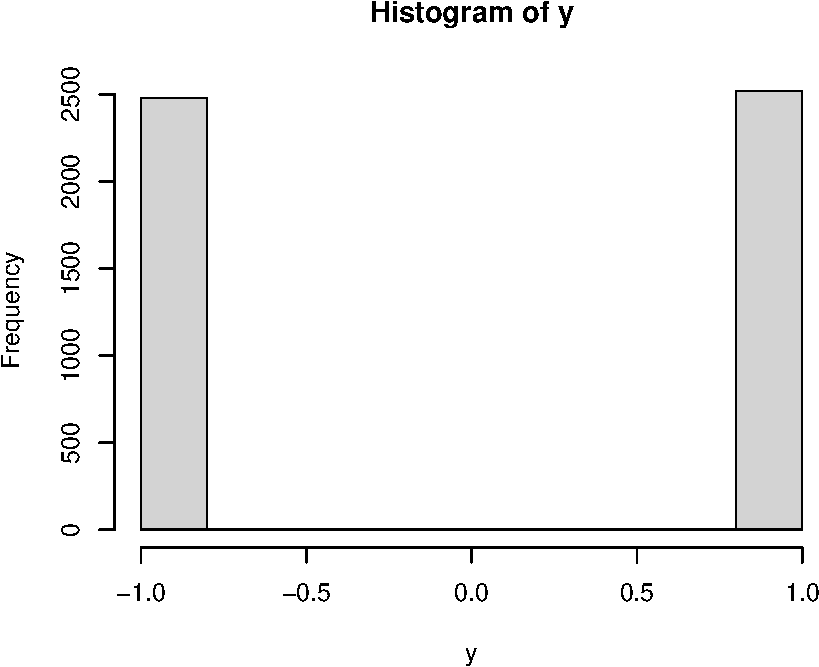
\includegraphics[width=1.5\linewidth]{TMA4268_2023_Exam_files/figure-latex/unnamed-chunk-1-1}

Given that \(\pi_0=\pi_1=0.5\), and the knowledge about the
class-specific distributions \(f_0(x)\) and \(f_1(x)\) given above, the
aim is to derive the equation for the Bayes decision boundary to find
the Bayes classifier.

\begin{enumerate}
\def\labelenumi{(\roman{enumi})}
\tightlist
\item
  (1P) Explain what the Bayes decision boundary actually is.
\item
  (3P) Write down the equation to be solved with the actual values (you
  are not supposed/asked to solve the equation), and explain what the
  unknowns are.
\item
  (1P) Is the resulting boundary linear in the covariates? Why?
\end{enumerate}

\textbf{Solution}:

\begin{enumerate}
\def\labelenumi{(\roman{enumi})}
\item
  Say either: The Bayes decision boundary is where the probabilities for
  the two classes are equal (0.5P for this), or: observations are
  classified to \emph{the most probable class} (the class with the
  highest posterior probability; 0.5P for this alternative argument).
  Using this boundary thus gives \emph{the minimum expected 0/1 loss}
  (0.5P for the last part, max 1P in total).
\item
  Here we need to find the equation where
\end{enumerate}

\[f_0(x)\pi_0 = f_1(x) \pi_1 \ , \] and since \(\pi_0=\pi_1\), we only
need to solve

\[f_0(x) = f_1(x)   \ . \] (1P if the students gets here). (Note that
log-transformation does not help much here due to the sum in the
likelihood for group 0.)

Thus, the equation is given as

\begin{align*}
0.5 & \cdot \frac{1}{2\pi |\Sigma|} \cdot \exp\left(- \frac{1}{2} (\bm{x}-\bm{\mu}_{01})^\top \Sigma^{-1} (\bm{x}- \bm{\mu}_{01})\right) + 0.5 \cdot \frac{1}{2\pi |\Sigma|} \cdot \exp\left( -\frac{1}{2} (\bm{x}-\bm{\mu}_{02})^\top \Sigma^{-1} (\bm{x}- \bm{\mu}_{02})\right)  \\
 = &   \frac{1}{2\pi |\Sigma|} \cdot \exp\left(-\frac{1}{2} (\bm{x}-\bm{\mu}_{2})^\top\Sigma^{-1}(\bm{x}-\bm{\mu}_{2})\right) \ ,
\end{align*}

(1P),

where the students are expected to plug in the actual values for
\(\bm{\mu}_{01}\), \(\bm{\mu}_{02}\), \(\Sigma\) etc. (1P for plugging
in the values)

\begin{enumerate}
\def\labelenumi{(\roman{enumi})}
\setcounter{enumi}{2}
\tightlist
\item
  No, the boundary is not linear (and neither quadratic) in the
  covariates, because by log-transforming we do not get rid of the
  exponential term due to the sum in group 0.
\end{enumerate}

\hypertarget{problem-3-data-analysis-1-regression-17p}{%
\section{Problem 3 -- Data analysis 1 -- regression
(17P)}\label{problem-3-data-analysis-1-regression-17p}}

Here we are looking at a regression problem, where we want to understand
the factors that affect birth weight of babies. We use the
\texttt{birthwt} data set from the MASS package, which you can load and
investigate using the code below and by typing \texttt{?birthwt} into
the R console:

\begin{Shaded}
\begin{Highlighting}[]
\FunctionTok{library}\NormalTok{(MASS)}
\FunctionTok{data}\NormalTok{(birthwt)}

\NormalTok{d.bw }\OtherTok{\textless{}{-}}\NormalTok{ birthwt}

\CommentTok{\# Race is a categorical variables, so we have to convert it:}
\NormalTok{d.bw}\SpecialCharTok{$}\NormalTok{race }\OtherTok{\textless{}{-}} \FunctionTok{as.factor}\NormalTok{(d.bw}\SpecialCharTok{$}\NormalTok{race)}

\CommentTok{\# Look at the data, for example using:}
\FunctionTok{pairs}\NormalTok{(d.bw)}
\end{Highlighting}
\end{Shaded}

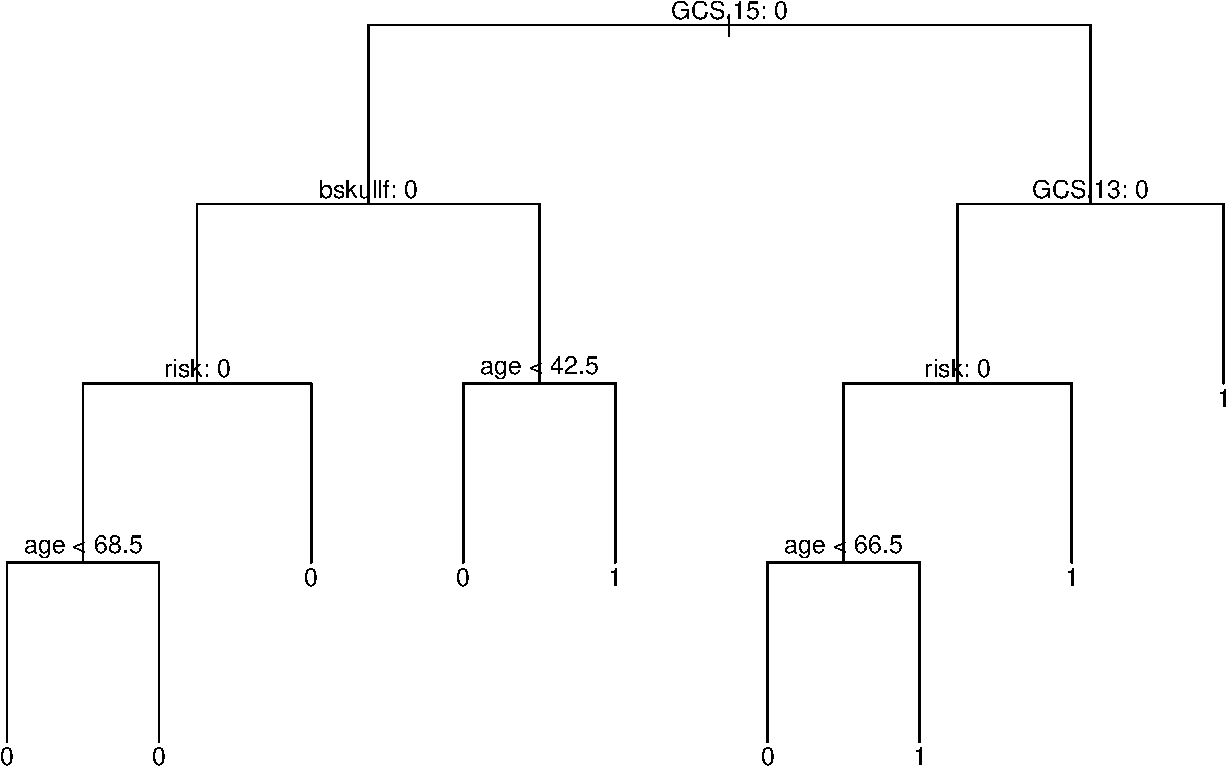
\includegraphics[width=0.8\linewidth]{TMA4268_2023_Exam_files/figure-latex/unnamed-chunk-2-1}

\begin{Shaded}
\begin{Highlighting}[]
\FunctionTok{str}\NormalTok{(d.bw)}
\end{Highlighting}
\end{Shaded}

\begin{verbatim}
## 'data.frame':    189 obs. of  10 variables:
##  $ low  : int  0 0 0 0 0 0 0 0 0 0 ...
##  $ age  : int  19 33 20 21 18 21 22 17 29 26 ...
##  $ lwt  : int  182 155 105 108 107 124 118 103 123 113 ...
##  $ race : Factor w/ 3 levels "1","2","3": 2 3 1 1 1 3 1 3 1 1 ...
##  $ smoke: int  0 0 1 1 1 0 0 0 1 1 ...
##  $ ptl  : int  0 0 0 0 0 0 0 0 0 0 ...
##  $ ht   : int  0 0 0 0 0 0 0 0 0 0 ...
##  $ ui   : int  1 0 0 1 1 0 0 0 0 0 ...
##  $ ftv  : int  0 3 1 2 0 0 1 1 1 0 ...
##  $ bwt  : int  2523 2551 2557 2594 2600 2622 2637 2637 2663 2665 ...
\end{verbatim}

In order to assess the robustness of our models, we split the data into
a training and a test set as follows:

\begin{Shaded}
\begin{Highlighting}[]
\FunctionTok{set.seed}\NormalTok{(}\DecValTok{1234}\NormalTok{)}
\NormalTok{samples }\OtherTok{\textless{}{-}} \FunctionTok{sample}\NormalTok{(}\DecValTok{1}\SpecialCharTok{:}\DecValTok{189}\NormalTok{, }\DecValTok{132}\NormalTok{, }\AttributeTok{replace =}\NormalTok{ F)}
\NormalTok{d.bw.train }\OtherTok{\textless{}{-}}\NormalTok{ d.bw[samples, ]}
\NormalTok{d.bw.test }\OtherTok{\textless{}{-}}\NormalTok{ d.bw[}\SpecialCharTok{{-}}\NormalTok{samples, ]}
\end{Highlighting}
\end{Shaded}

\hypertarget{a-4p}{%
\subsection{a) (4P)}\label{a-4p}}

\begin{enumerate}
\def\labelenumi{(\roman{enumi})}
\item
  (1P) Fit a linear regression model on the training data, where you use
  birth weight in grams (\texttt{bwt}) as the response and all variables
  \textbf{except \texttt{low}} as predictors. Report the regression
  coefficients, standard errors and \(p\)-values (use the standard way
  to do this in R).
\item
  (1P) What is the expected difference in birth weight for babies of
  black women compared to white women?
\item
  (1P) Is there evidence for \texttt{race} being relevant in the model?
  Say which test you carry out and report the respective \(p\)-value.
\item
  (1P) Compare \(R^2\) and \(R^2_{adj}\) of the model and interpret what
  you find.
\end{enumerate}

\textbf{Solution:} (i)

\begin{Shaded}
\begin{Highlighting}[]
\NormalTok{r.lm1 }\OtherTok{\textless{}{-}} \FunctionTok{lm}\NormalTok{(bwt }\SpecialCharTok{\textasciitilde{}}\NormalTok{ age }\SpecialCharTok{+}\NormalTok{ lwt }\SpecialCharTok{+}\NormalTok{ race }\SpecialCharTok{+}\NormalTok{ smoke }\SpecialCharTok{+}\NormalTok{ ptl }\SpecialCharTok{+}\NormalTok{ ht }\SpecialCharTok{+}\NormalTok{ ui }\SpecialCharTok{+}\NormalTok{ ftv, d.bw.train)}
\FunctionTok{summary}\NormalTok{(r.lm1)}
\end{Highlighting}
\end{Shaded}

\begin{verbatim}
## 
## Call:
## lm(formula = bwt ~ age + lwt + race + smoke + ptl + ht + ui + 
##     ftv, data = d.bw.train)
## 
## Residuals:
##      Min       1Q   Median       3Q      Max 
## -1676.18  -466.05    29.52   488.72  1772.87 
## 
## Coefficients:
##             Estimate Std. Error t value Pr(>|t|)    
## (Intercept) 2774.220    379.761   7.305 3.13e-11 ***
## age           -4.608     11.681  -0.394 0.693916    
## lwt            5.302      2.115   2.507 0.013500 *  
## race2       -532.557    181.592  -2.933 0.004014 ** 
## race3       -326.391    141.538  -2.306 0.022797 *  
## smoke       -264.044    133.499  -1.978 0.050197 .  
## ptl         -146.597    130.288  -1.125 0.262724    
## ht          -687.332    254.689  -2.699 0.007948 ** 
## ui          -628.922    169.085  -3.720 0.000303 ***
## ftv           -1.865     55.124  -0.034 0.973066    
## ---
## Signif. codes:  0 '***' 0.001 '**' 0.01 '*' 0.05 '.' 0.1 ' ' 1
## 
## Residual standard error: 667.4 on 122 degrees of freedom
## Multiple R-squared:  0.2695, Adjusted R-squared:  0.2157 
## F-statistic: 5.002 on 9 and 122 DF,  p-value: 9.836e-06
\end{verbatim}

\begin{enumerate}
\def\labelenumi{(\roman{enumi})}
\setcounter{enumi}{1}
\tightlist
\item
  -533 grams
\item
  F-test using the anova function in R:
\end{enumerate}

\begin{Shaded}
\begin{Highlighting}[]
\FunctionTok{anova}\NormalTok{(r.lm1)}
\end{Highlighting}
\end{Shaded}

\begin{verbatim}
## Analysis of Variance Table
## 
## Response: bwt
##            Df   Sum Sq Mean Sq F value    Pr(>F)    
## age         1   301426  301426  0.6768 0.4122979    
## lwt         1  3267325 3267325  7.3362 0.0077297 ** 
## race        2  3311398 1655699  3.7176 0.0270876 *  
## smoke       1  3332287 3332287  7.4820 0.0071615 ** 
## ptl         1  1016195 1016195  2.2817 0.1334964    
## ht          1  2655528 2655528  5.9625 0.0160476 *  
## ui          1  6165125 6165125 13.8426 0.0003018 ***
## ftv         1      510     510  0.0011 0.9730662    
## Residuals 122 54335487  445373                      
## ---
## Signif. codes:  0 '***' 0.001 '**' 0.01 '*' 0.05 '.' 0.1 ' ' 1
\end{verbatim}

The p-value is small (\textless0.05), thus yes, there is evidence.

\begin{enumerate}
\def\labelenumi{(\roman{enumi})}
\setcounter{enumi}{3}
\tightlist
\item
  The two values should be reported here: \(R^2=0.267\) and
  \(R^2_{adj}=0.216\). The difference in the two \(R^2\) values
  indicates that there are some unneccesary variables in the model.
  Note: Students don't need to interpret the \(R^2\) itself, only the
  differnces.
\end{enumerate}

\hypertarget{b-3p}{%
\subsection{b) (3P)}\label{b-3p}}

\begin{enumerate}
\def\labelenumi{(\roman{enumi})}
\tightlist
\item
  (2P) A medical researcher is interested to know whether the effect of
  the mother's smoking status during pregnancy changes with the age of
  the mother. Expand the model from a) such that it accounts for the
  possibility that the effect of smoking depends on age and interpret
  the results, still using the training data. In particular, answer the
  question of the researcher and compare \(R^2\) to the one from a).
\item
  (1P) According to your modeling output, when the mother is smoking,
  how much does the expected birth weight change for a mother age 35
  compared to a mother age 25, given that all other variables are the
  same?
\end{enumerate}

\textbf{Solution}

\begin{enumerate}
\def\labelenumi{(\roman{enumi})}
\tightlist
\item
  The model and its output are as follows (1P for the correct model, no
  point if the interaction is lacking and -0.5P for other mistakes):
\end{enumerate}

\begin{Shaded}
\begin{Highlighting}[]
\NormalTok{r.lm2 }\OtherTok{\textless{}{-}} \FunctionTok{lm}\NormalTok{(bwt }\SpecialCharTok{\textasciitilde{}}\NormalTok{ age }\SpecialCharTok{+}\NormalTok{ lwt }\SpecialCharTok{+}\NormalTok{ race }\SpecialCharTok{+}\NormalTok{ ptl }\SpecialCharTok{+}\NormalTok{ ht }\SpecialCharTok{+}\NormalTok{ ui }\SpecialCharTok{+}\NormalTok{ ftv }\SpecialCharTok{+}\NormalTok{ smoke }\SpecialCharTok{*}\NormalTok{ age,}
\NormalTok{    d.bw.train)}
\FunctionTok{summary}\NormalTok{(r.lm2)}
\end{Highlighting}
\end{Shaded}

\begin{verbatim}
## 
## Call:
## lm(formula = bwt ~ age + lwt + race + ptl + ht + ui + ftv + smoke * 
##     age, data = d.bw.train)
## 
## Residuals:
##      Min       1Q   Median       3Q      Max 
## -1696.40  -518.00    26.93   516.30  1398.18 
## 
## Coefficients:
##             Estimate Std. Error t value Pr(>|t|)    
## (Intercept) 2286.122    427.968   5.342 4.39e-07 ***
## age           14.421     14.089   1.024  0.30810    
## lwt            5.268      2.078   2.535  0.01251 *  
## race2       -451.590    181.752  -2.485  0.01433 *  
## race3       -268.483    141.252  -1.901  0.05972 .  
## ptl         -131.475    128.156  -1.026  0.30699    
## ht          -676.711    250.241  -2.704  0.00783 ** 
## ui          -689.382    168.124  -4.100 7.50e-05 ***
## ftv            8.813     54.347   0.162  0.87145    
## smoke       1044.110    577.136   1.809  0.07291 .  
## age:smoke    -55.732     23.945  -2.328  0.02160 *  
## ---
## Signif. codes:  0 '***' 0.001 '**' 0.01 '*' 0.05 '.' 0.1 ' ' 1
## 
## Residual standard error: 655.6 on 121 degrees of freedom
## Multiple R-squared:  0.3008, Adjusted R-squared:  0.2431 
## F-statistic: 5.207 on 10 and 121 DF,  p-value: 2.483e-06
\end{verbatim}

Interpretation: Yes, the effect of smoking changes with age (0.5P).
Older women have an even higher risk of low birth weight when they smoke
than younger women. The \(R^2=0.30\) has clearly improved, underlining
that the interaction term is relevant (0.5P).

\begin{enumerate}
\def\labelenumi{(\roman{enumi})}
\setcounter{enumi}{1}
\tightlist
\item
  The overall effect of age is given by
  \(\beta_{age} + \beta_{age:smoking}\), thus we have to multiply this
  term by 10 to obtain the expected reduction in birth weight: -413.1.
  Here there is an all-or-nothing grading (1P for correct value, 0P
  otherwise).
\end{enumerate}

\hypertarget{c-3p}{%
\subsection{c) (3P)}\label{c-3p}}

\begin{enumerate}
\def\labelenumi{(\roman{enumi})}
\tightlist
\item
  (1P) Carry out Lasso regression on the training set excluding the
  variable \texttt{low} (like in a) and b)), and say how you choose
  \(\lambda\).
\item
  (2P) Compare the regression coefficients from the Lasso with those
  from the linear regression in a). What pattern(s) do you notice? Would
  you see the same if you had carried out ridge regression?
\end{enumerate}

\textbf{R-hints}:

\begin{Shaded}
\begin{Highlighting}[]
\NormalTok{x.train }\OtherTok{\textless{}{-}} \FunctionTok{model.matrix}\NormalTok{(bwt }\SpecialCharTok{\textasciitilde{}}\NormalTok{ . }\SpecialCharTok{{-}}\NormalTok{ low, }\AttributeTok{data =}\NormalTok{ d.bw.train)[, }\SpecialCharTok{{-}}\DecValTok{1}\NormalTok{]}
\NormalTok{y.train }\OtherTok{\textless{}{-}}\NormalTok{ d.bw.train}\SpecialCharTok{$}\NormalTok{bwt}
\NormalTok{x.test }\OtherTok{=} \FunctionTok{model.matrix}\NormalTok{(bwt }\SpecialCharTok{\textasciitilde{}}\NormalTok{ . }\SpecialCharTok{{-}}\NormalTok{ low, }\AttributeTok{data =}\NormalTok{ d.bw.test)[, }\SpecialCharTok{{-}}\DecValTok{1}\NormalTok{]}
\NormalTok{y.test }\OtherTok{=}\NormalTok{ d.bw.test}\SpecialCharTok{$}\NormalTok{bwt}
\end{Highlighting}
\end{Shaded}

\begin{Shaded}
\begin{Highlighting}[]
\FunctionTok{library}\NormalTok{(glmnet)}
\FunctionTok{set.seed}\NormalTok{(}\DecValTok{10}\NormalTok{)}
\NormalTok{cv.lasso }\OtherTok{\textless{}{-}} \FunctionTok{cv.glmnet}\NormalTok{(x.train, y.train, }\AttributeTok{alpha =}\NormalTok{ ...)}
\FunctionTok{plot}\NormalTok{(cv.lasso)}
\NormalTok{cv.lasso}\SpecialCharTok{$}\NormalTok{...}
\NormalTok{bw.lasso }\OtherTok{\textless{}{-}} \FunctionTok{glmnet}\NormalTok{(..., ..., }\AttributeTok{alpha =}\NormalTok{ ..., }\AttributeTok{lambda =}\NormalTok{ ...)}
\end{Highlighting}
\end{Shaded}

\textbf{Solution}

\begin{enumerate}
\def\labelenumi{(\roman{enumi})}
\tightlist
\item
\end{enumerate}

\begin{Shaded}
\begin{Highlighting}[]
\FunctionTok{library}\NormalTok{(glmnet)}
\FunctionTok{set.seed}\NormalTok{(}\DecValTok{10}\NormalTok{)}
\NormalTok{cv.lasso }\OtherTok{\textless{}{-}} \FunctionTok{cv.glmnet}\NormalTok{(x.train, y.train, }\AttributeTok{alpha =} \DecValTok{1}\NormalTok{)}
\FunctionTok{plot}\NormalTok{(cv.lasso)}
\end{Highlighting}
\end{Shaded}

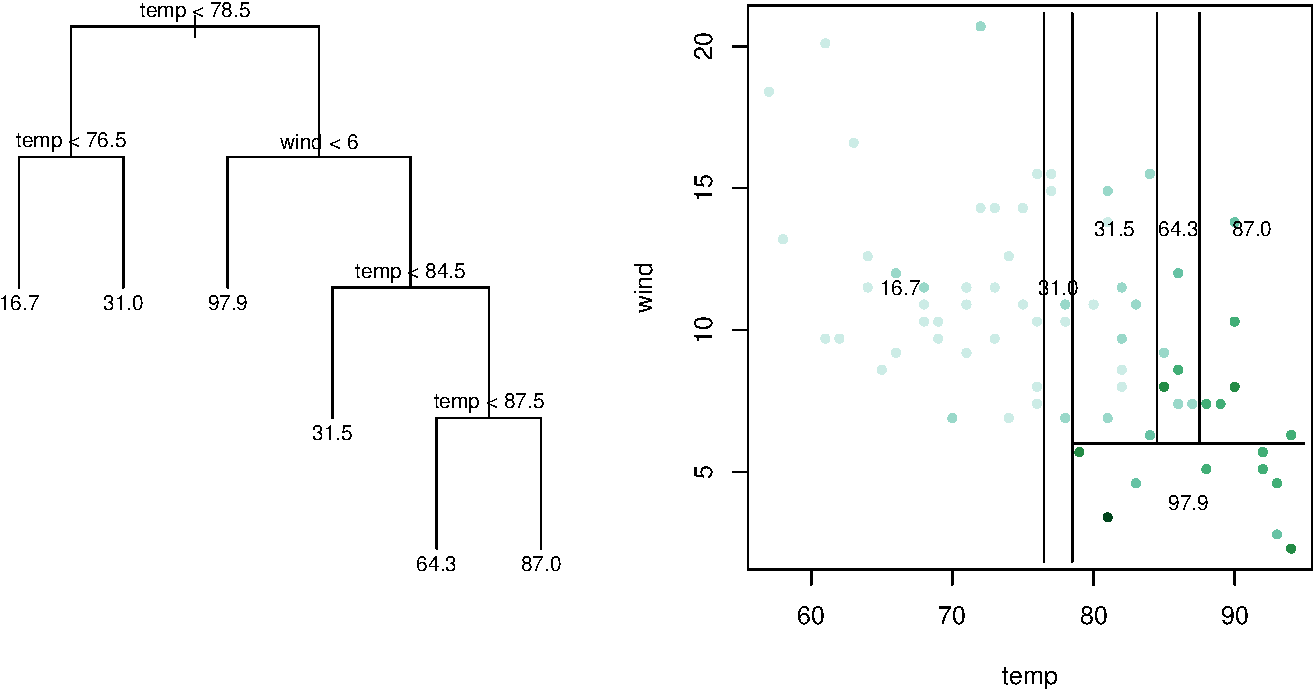
\includegraphics{TMA4268_2023_Exam_files/figure-latex/unnamed-chunk-9-1.pdf}

\begin{Shaded}
\begin{Highlighting}[]
\NormalTok{cv.lasso}\SpecialCharTok{$}\NormalTok{lambda.min}
\end{Highlighting}
\end{Shaded}

\begin{verbatim}
## [1] 23.55878
\end{verbatim}

\begin{Shaded}
\begin{Highlighting}[]
\NormalTok{bw.lasso }\OtherTok{\textless{}{-}} \FunctionTok{glmnet}\NormalTok{(x.train, y.train, }\AttributeTok{alpha =} \DecValTok{1}\NormalTok{, }\AttributeTok{lambda =}\NormalTok{ cv.lasso}\SpecialCharTok{$}\NormalTok{lambda.min)}

\FunctionTok{coef}\NormalTok{(bw.lasso)}
\end{Highlighting}
\end{Shaded}

\begin{verbatim}
## 10 x 1 sparse Matrix of class "dgCMatrix"
##                      s0
## (Intercept) 2685.110986
## age            .       
## lwt            4.337968
## race2       -396.970442
## race3       -225.086479
## smoke       -187.480612
## ptl         -129.089274
## ht          -552.987923
## ui          -573.098758
## ftv            .
\end{verbatim}

Alternatively, with \texttt{lambda.1se}:

\begin{Shaded}
\begin{Highlighting}[]
\NormalTok{cv.lasso}\SpecialCharTok{$}\NormalTok{lambda}\FloatTok{.1}\NormalTok{se}
\end{Highlighting}
\end{Shaded}

\begin{verbatim}
## [1] 104.38
\end{verbatim}

\begin{Shaded}
\begin{Highlighting}[]
\NormalTok{bw.lasso}\FloatTok{.1}\NormalTok{se }\OtherTok{\textless{}{-}} \FunctionTok{glmnet}\NormalTok{(x.train, y.train, }\AttributeTok{alpha =} \DecValTok{1}\NormalTok{, }\AttributeTok{lambda =}\NormalTok{ cv.lasso}\SpecialCharTok{$}\NormalTok{lambda}\FloatTok{.1}\NormalTok{se)}

\FunctionTok{coef}\NormalTok{(bw.lasso}\FloatTok{.1}\NormalTok{se)}
\end{Highlighting}
\end{Shaded}

\begin{verbatim}
## 10 x 1 sparse Matrix of class "dgCMatrix"
##                      s0
## (Intercept) 2778.223411
## age            .       
## lwt            1.446888
## race2        -20.086476
## race3          .       
## smoke          .       
## ptl          -31.634403
## ht          -121.384488
## ui          -374.208781
## ftv            .
\end{verbatim}

\(\lambda\) is chosen using cross-validation (0.5P).

\begin{enumerate}
\def\labelenumi{(\roman{enumi})}
\setcounter{enumi}{1}
\tightlist
\item
  There are two patterns to notice: The coefficients are shrunken (0.5P)
  and some are zero (0.5P). For ridge we would also have expected to see
  shrinkage (0.5P), but none of the coefficients had gone to zero
  (0.5P). Here I expect to explicitly hint that the coefficients are
  getting smaller/shurunken (not just that some are close to zero for
  ridge, for example).
\end{enumerate}

\hypertarget{d-3p}{%
\subsection{d) (3P)}\label{d-3p}}

Report the MSEs for the test set for all the models fit in a), b) and
c). Which method performs best?

\textbf{Solution: }

\begin{Shaded}
\begin{Highlighting}[]
\NormalTok{r.lm1 }\OtherTok{\textless{}{-}} \FunctionTok{lm}\NormalTok{(bwt }\SpecialCharTok{\textasciitilde{}}\NormalTok{ age }\SpecialCharTok{+}\NormalTok{ lwt }\SpecialCharTok{+}\NormalTok{ race }\SpecialCharTok{+}\NormalTok{ smoke }\SpecialCharTok{+}\NormalTok{ ptl }\SpecialCharTok{+}\NormalTok{ ht }\SpecialCharTok{+}\NormalTok{ ui }\SpecialCharTok{+}\NormalTok{ ftv, d.bw.train)}
\NormalTok{r.pred.lm1 }\OtherTok{\textless{}{-}} \FunctionTok{predict}\NormalTok{(r.lm1, }\AttributeTok{newdata =}\NormalTok{ d.bw.test)}
\NormalTok{mse.a }\OtherTok{\textless{}{-}} \FunctionTok{mean}\NormalTok{((r.pred.lm1 }\SpecialCharTok{{-}}\NormalTok{ d.bw.test}\SpecialCharTok{$}\NormalTok{bwt)}\SpecialCharTok{\^{}}\DecValTok{2}\NormalTok{)}

\NormalTok{r.lm2 }\OtherTok{\textless{}{-}} \FunctionTok{lm}\NormalTok{(bwt }\SpecialCharTok{\textasciitilde{}}\NormalTok{ age }\SpecialCharTok{+}\NormalTok{ lwt }\SpecialCharTok{+}\NormalTok{ race }\SpecialCharTok{+}\NormalTok{ smoke }\SpecialCharTok{*}\NormalTok{ age }\SpecialCharTok{+}\NormalTok{ ptl }\SpecialCharTok{+}\NormalTok{ ht }\SpecialCharTok{+}\NormalTok{ ui }\SpecialCharTok{+}\NormalTok{ ftv,}
\NormalTok{    d.bw.train)}
\NormalTok{r.pred.lm2 }\OtherTok{\textless{}{-}} \FunctionTok{predict}\NormalTok{(r.lm2, }\AttributeTok{newdata =}\NormalTok{ d.bw.test)}
\NormalTok{mse.b }\OtherTok{\textless{}{-}} \FunctionTok{mean}\NormalTok{((r.pred.lm2 }\SpecialCharTok{{-}}\NormalTok{ d.bw.test}\SpecialCharTok{$}\NormalTok{bwt)}\SpecialCharTok{\^{}}\DecValTok{2}\NormalTok{)}

\NormalTok{r.lasso }\OtherTok{\textless{}{-}} \FunctionTok{predict}\NormalTok{(bw.lasso, }\AttributeTok{newx =}\NormalTok{ x.test)}
\NormalTok{mse.c }\OtherTok{\textless{}{-}} \FunctionTok{mean}\NormalTok{((r.lasso }\SpecialCharTok{{-}}\NormalTok{ d.bw.test}\SpecialCharTok{$}\NormalTok{bwt)}\SpecialCharTok{\^{}}\DecValTok{2}\NormalTok{)}

\CommentTok{\# Also for the case where the larger lambda is used in d):}
\NormalTok{r.lasso}\FloatTok{.1}\NormalTok{se }\OtherTok{\textless{}{-}} \FunctionTok{predict}\NormalTok{(bw.lasso}\FloatTok{.1}\NormalTok{se, }\AttributeTok{newx =}\NormalTok{ x.test)}
\NormalTok{mse.c}\FloatTok{.1}\NormalTok{se }\OtherTok{\textless{}{-}} \FunctionTok{mean}\NormalTok{((r.lasso}\FloatTok{.1}\NormalTok{se }\SpecialCharTok{{-}}\NormalTok{ d.bw.test}\SpecialCharTok{$}\NormalTok{bwt)}\SpecialCharTok{\^{}}\DecValTok{2}\NormalTok{)}

\FunctionTok{c}\NormalTok{(mse.a, mse.b, mse.c, mse.c}\FloatTok{.1}\NormalTok{se)}
\end{Highlighting}
\end{Shaded}

\begin{verbatim}
## [1] 406158.6 417858.8 396418.9 431157.5
\end{verbatim}

Lasso performs best if lambda.min was used, otherwise standard
regression performs best.

\hypertarget{e-4p}{%
\subsection{e) (4P)}\label{e-4p}}

Finally choose a more flexible method than those used above to find a
model with \emph{lower test error}. Explain your model and the choices
you make. Code without explanation will not give full score.

\textbf{R-hints:}

\begin{Shaded}
\begin{Highlighting}[]
\FunctionTok{library}\NormalTok{(gam)}
\FunctionTok{library}\NormalTok{(randomForest)}
\end{Highlighting}
\end{Shaded}

\textbf{Solution: }

Here there is a lot of freedom. The students will probably use a GAM or
a regression tree.

In a regression tree, the students must explain the choice for the
number of trees and mtry (if either is lacking, -1P for each). It's not
enough to say ``I choose the default no of trees from the
lecture/function'' or ``I chose ntree=500'', for example -- ntrees
should be chosen \emph{large enough} (i.e., it is no tuning parameter),
and that should be made clear. Note that ntrees is not a tuning
parameter, so the students should not optimize it. If students choose a
GAM, they also need to explain each term and the choices they made.

Here is one solution: The idea is to use only variables that are left
from the Lasso and then apply a cubic spline on the only continuous
variable \texttt{lwt}:

\begin{Shaded}
\begin{Highlighting}[]
\FunctionTok{library}\NormalTok{(gam)}
\NormalTok{r.gam }\OtherTok{\textless{}{-}} \FunctionTok{gam}\NormalTok{(bwt }\SpecialCharTok{\textasciitilde{}} \FunctionTok{bs}\NormalTok{(lwt, }\DecValTok{4}\NormalTok{) }\SpecialCharTok{+}\NormalTok{ race }\SpecialCharTok{+}\NormalTok{ smoke }\SpecialCharTok{+}\NormalTok{ ptl }\SpecialCharTok{+}\NormalTok{ ht }\SpecialCharTok{+}\NormalTok{ ui, }\AttributeTok{data =}\NormalTok{ d.bw.train)}
\NormalTok{r.pred.gam }\OtherTok{\textless{}{-}} \FunctionTok{predict}\NormalTok{(r.gam, }\AttributeTok{newdata =}\NormalTok{ d.bw.test)}
\FunctionTok{mean}\NormalTok{((r.pred.gam }\SpecialCharTok{{-}}\NormalTok{ d.bw.test}\SpecialCharTok{$}\NormalTok{bwt)}\SpecialCharTok{\^{}}\DecValTok{2}\NormalTok{)}
\end{Highlighting}
\end{Shaded}

\begin{verbatim}
## [1] 392554.2
\end{verbatim}

Here is a solution with random forests. Note that the students then need
to explain \texttt{mtry} (usually p/3 for regression problems) and say
that number of trees must be ``large enough''.

\begin{Shaded}
\begin{Highlighting}[]
\FunctionTok{library}\NormalTok{(randomForest)}
\NormalTok{rf.model }\OtherTok{\textless{}{-}} \FunctionTok{randomForest}\NormalTok{(x.train, y.train, }\AttributeTok{mtry =} \DecValTok{3}\NormalTok{, }\AttributeTok{ntree =} \DecValTok{500}\NormalTok{)}
\NormalTok{yhat.rf }\OtherTok{\textless{}{-}} \FunctionTok{predict}\NormalTok{(rf.model, }\AttributeTok{newdata =}\NormalTok{ x.test)}
\NormalTok{(}\FunctionTok{mean}\NormalTok{((yhat.rf }\SpecialCharTok{{-}}\NormalTok{ y.test)}\SpecialCharTok{\^{}}\DecValTok{2}\NormalTok{))}
\end{Highlighting}
\end{Shaded}

\begin{verbatim}
## [1] 350918.7
\end{verbatim}

\clearpage

\hypertarget{problem-4-data-analysis-2-classification-12p}{%
\section{Problem 4 -- Data analysis 2 -- classification
(12P)}\label{problem-4-data-analysis-2-classification-12p}}

We look at the same data set as in Problem 3. Use the same code to load
and prepare the data:

\begin{Shaded}
\begin{Highlighting}[]
\FunctionTok{library}\NormalTok{(MASS)}
\FunctionTok{data}\NormalTok{(birthwt)}

\NormalTok{d.bw }\OtherTok{\textless{}{-}}\NormalTok{ birthwt}

\CommentTok{\# Race is a categorical variables, so we have to convert it:}
\NormalTok{d.bw}\SpecialCharTok{$}\NormalTok{race }\OtherTok{\textless{}{-}} \FunctionTok{as.factor}\NormalTok{(d.bw}\SpecialCharTok{$}\NormalTok{race)}
\CommentTok{\# Also convert low for later use:}
\NormalTok{d.bw}\SpecialCharTok{$}\NormalTok{low }\OtherTok{\textless{}{-}} \FunctionTok{as.factor}\NormalTok{(d.bw}\SpecialCharTok{$}\NormalTok{low)}
\end{Highlighting}
\end{Shaded}

In order to assess the robustness of our models, we split the data into
a training and a test set as follows:

\begin{Shaded}
\begin{Highlighting}[]
\FunctionTok{set.seed}\NormalTok{(}\DecValTok{1234}\NormalTok{)}
\NormalTok{samples }\OtherTok{\textless{}{-}} \FunctionTok{sample}\NormalTok{(}\DecValTok{1}\SpecialCharTok{:}\DecValTok{189}\NormalTok{, }\DecValTok{132}\NormalTok{, }\AttributeTok{replace =}\NormalTok{ F)}
\NormalTok{d.bw.train }\OtherTok{\textless{}{-}}\NormalTok{ d.bw[samples, ]}
\NormalTok{d.bw.test }\OtherTok{\textless{}{-}}\NormalTok{ d.bw[}\SpecialCharTok{{-}}\NormalTok{samples, ]}
\end{Highlighting}
\end{Shaded}

The aim is to both \emph{understand} why and \emph{predict} whether a
newborn baby has low birthweight (\(<2.5kg\)), using the binary
indicator variable \texttt{low} for being underweight.

\hypertarget{a-3p}{%
\subsection{a) (3P)}\label{a-3p}}

\begin{enumerate}
\def\labelenumi{(\roman{enumi})}
\item
  (1P) Fit a logistic regression model that can be used to predict
  whether a baby will be underweight, including all predictor variables
  \textbf{except \texttt{bwt}} as predictors. Report the coefficients,
  standard errors and \(p\)-values (use the standard way to do this in
  R).
\item
  (2P) Report the probability to give birth to an underweight baby for a
  female with the following characteristics:
\end{enumerate}

\begin{itemize}
\tightlist
\item
  age=25
\item
  lwt (weight in pounds)=155
\item
  race=white
\item
  smoke = 1 (yes)
\item
  ptl=0
\item
  ht=0
\item
  ui=0
\item
  ftw=1
\end{itemize}

\textbf{R-hints:}

\begin{Shaded}
\begin{Highlighting}[]
\FunctionTok{glm}\NormalTok{(..., }\AttributeTok{family =} \StringTok{"binomial"}\NormalTok{)}
\end{Highlighting}
\end{Shaded}

\textbf{Solution:}

\begin{Shaded}
\begin{Highlighting}[]
\NormalTok{r.glm }\OtherTok{\textless{}{-}} \FunctionTok{glm}\NormalTok{(low }\SpecialCharTok{\textasciitilde{}}\NormalTok{ age }\SpecialCharTok{+}\NormalTok{ lwt }\SpecialCharTok{+}\NormalTok{ race }\SpecialCharTok{+}\NormalTok{ smoke }\SpecialCharTok{+}\NormalTok{ ptl }\SpecialCharTok{+}\NormalTok{ ht }\SpecialCharTok{+}\NormalTok{ ui }\SpecialCharTok{+}\NormalTok{ ftv, d.bw.train,}
    \AttributeTok{family =} \StringTok{"binomial"}\NormalTok{)}
\FunctionTok{summary}\NormalTok{(r.glm)}
\end{Highlighting}
\end{Shaded}

\begin{verbatim}
## 
## Call:
## glm(formula = low ~ age + lwt + race + smoke + ptl + ht + ui + 
##     ftv, family = "binomial", data = d.bw.train)
## 
## Deviance Residuals: 
##     Min       1Q   Median       3Q      Max  
## -1.5624  -0.8019  -0.5389   0.9842   2.2859  
## 
## Coefficients:
##               Estimate Std. Error z value Pr(>|z|)  
## (Intercept)  1.2626642  1.4627818   0.863   0.3880  
## age         -0.0305166  0.0437289  -0.698   0.4853  
## lwt         -0.0185549  0.0085725  -2.164   0.0304 *
## race2        1.3220153  0.6171069   2.142   0.0322 *
## race3        0.5436934  0.5362748   1.014   0.3107  
## smoke        0.5196261  0.4905968   1.059   0.2895  
## ptl          0.8310422  0.4422122   1.879   0.0602 .
## ht           2.1264726  0.9010048   2.360   0.0183 *
## ui           1.1355797  0.5468967   2.076   0.0379 *
## ftv         -0.0006133  0.2035747  -0.003   0.9976  
## ---
## Signif. codes:  0 '***' 0.001 '**' 0.01 '*' 0.05 '.' 0.1 ' ' 1
## 
## (Dispersion parameter for binomial family taken to be 1)
## 
##     Null deviance: 169.39  on 131  degrees of freedom
## Residual deviance: 142.45  on 122  degrees of freedom
## AIC: 162.45
## 
## Number of Fisher Scoring iterations: 4
\end{verbatim}

\begin{enumerate}
\def\labelenumi{(\roman{enumi})}
\setcounter{enumi}{1}
\tightlist
\item
  One way to implement this is as follows (but you can also use the
  \texttt{predict()} function):
\end{enumerate}

\begin{Shaded}
\begin{Highlighting}[]
\NormalTok{x.data }\OtherTok{\textless{}{-}} \FunctionTok{c}\NormalTok{(}\DecValTok{1}\NormalTok{, }\DecValTok{25}\NormalTok{, }\DecValTok{155}\NormalTok{, }\DecValTok{0}\NormalTok{, }\DecValTok{0}\NormalTok{, }\DecValTok{1}\NormalTok{, }\DecValTok{0}\NormalTok{, }\DecValTok{0}\NormalTok{, }\DecValTok{0}\NormalTok{, }\DecValTok{1}\NormalTok{)}

\NormalTok{eta }\OtherTok{\textless{}{-}} \FunctionTok{t}\NormalTok{(}\FunctionTok{coef}\NormalTok{(r.glm)) }\SpecialCharTok{\%*\%}\NormalTok{ x.data}

\NormalTok{(prob }\OtherTok{\textless{}{-}} \FunctionTok{exp}\NormalTok{(eta)}\SpecialCharTok{/}\NormalTok{(}\DecValTok{1} \SpecialCharTok{+} \FunctionTok{exp}\NormalTok{(eta)))}
\end{Highlighting}
\end{Shaded}

\begin{verbatim}
##           [,1]
## [1,] 0.1350238
\end{verbatim}

The probability is 0.135.

\hypertarget{b-4p}{%
\subsection{b) (4P)}\label{b-4p}}

\begin{enumerate}
\def\labelenumi{(\roman{enumi})}
\item
  (2P) A medical doctor is interested in the overall effect that smoking
  has on low birth weight, based on logistic regression. Use the
  regression output from a) and explain to the doctor how smoking
  affects the chance for low birth weight. We are interested in a
  general statement that is not dependent on the value of the other
  variables.
\item
  (1P) Report the error rate for the test data using the fitted model
  from a).
\item
  (1P) Calculate sensitivity and specificity for the test data.
\end{enumerate}

\textbf{R-hints:}

\begin{Shaded}
\begin{Highlighting}[]
\FunctionTok{glm}\NormalTok{(..., }\AttributeTok{family =} \StringTok{"binomial"}\NormalTok{)}
\FunctionTok{predict}\NormalTok{(...)}
\FunctionTok{confusionMatrix}\NormalTok{(}\AttributeTok{data =}\NormalTok{ ..., }\AttributeTok{reference =}\NormalTok{ ...)}\SpecialCharTok{$}\NormalTok{table}
\end{Highlighting}
\end{Shaded}

\textbf{Solution:}

\begin{enumerate}
\def\labelenumi{(\roman{enumi})}
\tightlist
\item
  Here the students must NOT repeat the analysis from (a) with smoke=0,
  but look at the odds-ratio:
\end{enumerate}

\begin{Shaded}
\begin{Highlighting}[]
\FunctionTok{exp}\NormalTok{(}\FunctionTok{coef}\NormalTok{(r.glm)[}\StringTok{"smoke"}\NormalTok{])}
\end{Highlighting}
\end{Shaded}

\begin{verbatim}
##    smoke 
## 1.681399
\end{verbatim}

Interpretation: The odds for low birth weight increases by a
\emph{factor} of 1.68 for smoking women compared to non-smoking women.

\begin{enumerate}
\def\labelenumi{(\roman{enumi})}
\setcounter{enumi}{1}
\tightlist
\item
\end{enumerate}

\begin{Shaded}
\begin{Highlighting}[]
\NormalTok{t.pred.glm }\OtherTok{\textless{}{-}} \FunctionTok{round}\NormalTok{(}\FunctionTok{predict}\NormalTok{(r.glm, }\AttributeTok{newdata =}\NormalTok{ d.bw.test, }\AttributeTok{type =} \StringTok{"response"}\NormalTok{),}
    \DecValTok{0}\NormalTok{)}

\NormalTok{(confMat }\OtherTok{\textless{}{-}} \FunctionTok{confusionMatrix}\NormalTok{(}\AttributeTok{data =} \FunctionTok{as.factor}\NormalTok{(t.pred.glm), }\AttributeTok{reference =} \FunctionTok{as.factor}\NormalTok{(d.bw.test}\SpecialCharTok{$}\NormalTok{low))}\SpecialCharTok{$}\NormalTok{table)}
\end{Highlighting}
\end{Shaded}

\begin{verbatim}
##           Reference
## Prediction  0  1
##          0 36  8
##          1  7  6
\end{verbatim}

\begin{Shaded}
\begin{Highlighting}[]
\DecValTok{1} \SpecialCharTok{{-}}\NormalTok{ (}\FunctionTok{sum}\NormalTok{(}\FunctionTok{diag}\NormalTok{(confMat))}\SpecialCharTok{/}\FunctionTok{sum}\NormalTok{(confMat[}\DecValTok{1}\SpecialCharTok{:}\DecValTok{2}\NormalTok{, }\DecValTok{1}\SpecialCharTok{:}\DecValTok{2}\NormalTok{]))}
\end{Highlighting}
\end{Shaded}

\begin{verbatim}
## [1] 0.2631579
\end{verbatim}

\begin{enumerate}
\def\labelenumi{(\roman{enumi})}
\setcounter{enumi}{2}
\tightlist
\item
  Sensitivity: Corresponds to \(P(\hat{y}=1 | y=1)\), where \(y\) is the
  true (reference) value, thus 0.429. Specificity: Corresponds to
  \(P(\hat{y}=0 | y=0)\), thus 0.837.
\end{enumerate}

\hypertarget{c-5p}{%
\subsection{c) (5P)}\label{c-5p}}

As a comparison to the logistic regression model we are now using a
random forest.

\begin{enumerate}
\def\labelenumi{(\roman{enumi})}
\tightlist
\item
  (2P) Use a random forest to fit a model on the training data. Justify
  the choice of any parameters that you use.
\item
  (3P) Report the misclassification error (1P) sensitivity and
  specificity (1P) and compare the values to the logistic regression
  model above. Which of the methods is preferable and why (1P)?
\end{enumerate}

\textbf{R-hints}:

\begin{Shaded}
\begin{Highlighting}[]
\FunctionTok{library}\NormalTok{(randomForest)}
\FunctionTok{set.seed}\NormalTok{(}\DecValTok{4268}\NormalTok{)}

\FunctionTok{randomForest}\NormalTok{(...)}
\end{Highlighting}
\end{Shaded}

\textbf{Solution}:

\begin{enumerate}
\def\labelenumi{(\roman{enumi})}
\tightlist
\item
  1P to fit the model:
\end{enumerate}

\begin{Shaded}
\begin{Highlighting}[]
\FunctionTok{library}\NormalTok{(randomForest)}
\FunctionTok{set.seed}\NormalTok{(}\DecValTok{4268}\NormalTok{)}

\NormalTok{rf.bw }\OtherTok{=} \FunctionTok{randomForest}\NormalTok{(low }\SpecialCharTok{\textasciitilde{}}\NormalTok{ age }\SpecialCharTok{+}\NormalTok{ lwt }\SpecialCharTok{+}\NormalTok{ race }\SpecialCharTok{+}\NormalTok{ smoke }\SpecialCharTok{+}\NormalTok{ ptl }\SpecialCharTok{+}\NormalTok{ ht }\SpecialCharTok{+}\NormalTok{ ui }\SpecialCharTok{+}
\NormalTok{    ftv, }\AttributeTok{data =}\NormalTok{ d.bw.train, }\AttributeTok{mtry =} \DecValTok{2}\NormalTok{, }\AttributeTok{ntree =} \DecValTok{1000}\NormalTok{, }\AttributeTok{importance =} \ConstantTok{TRUE}\NormalTok{)}
\end{Highlighting}
\end{Shaded}

The most critical choice is \texttt{mtry}. Since we have 8 variables,
and \(\sqrt{8}=2.8\), we can choose \texttt{mtry} =2 or =3. Both are ok,
but need to be justified (0.5P). The number of trees is less critical
but needs to be ``large enough'' (0.5P for the argument).

\begin{enumerate}
\def\labelenumi{(\roman{enumi})}
\setcounter{enumi}{1}
\tightlist
\item
\end{enumerate}

\begin{Shaded}
\begin{Highlighting}[]
\NormalTok{t.pred.rf }\OtherTok{\textless{}{-}} \FunctionTok{as.factor}\NormalTok{(}\FunctionTok{predict}\NormalTok{(rf.bw, d.bw.test, }\AttributeTok{type =} \StringTok{"class"}\NormalTok{))}
\NormalTok{(confMat.rf }\OtherTok{\textless{}{-}} \FunctionTok{confusionMatrix}\NormalTok{(}\AttributeTok{data =}\NormalTok{ t.pred.rf, }\AttributeTok{reference =}\NormalTok{ d.bw.test}\SpecialCharTok{$}\NormalTok{low)}\SpecialCharTok{$}\NormalTok{table)}
\end{Highlighting}
\end{Shaded}

\begin{verbatim}
##           Reference
## Prediction  0  1
##          0 40 11
##          1  3  3
\end{verbatim}

\begin{Shaded}
\begin{Highlighting}[]
\DecValTok{1} \SpecialCharTok{{-}}\NormalTok{ (}\FunctionTok{sum}\NormalTok{(}\FunctionTok{diag}\NormalTok{(confMat.rf))}\SpecialCharTok{/}\FunctionTok{sum}\NormalTok{(confMat.rf[}\DecValTok{1}\SpecialCharTok{:}\DecValTok{2}\NormalTok{, }\DecValTok{1}\SpecialCharTok{:}\DecValTok{2}\NormalTok{]))}
\end{Highlighting}
\end{Shaded}

\begin{verbatim}
## [1] 0.245614
\end{verbatim}

Sensitivity: Corresponds to \(P(\hat{y}=1 | y=1)\) where \(y\) is the
true (reference) value, thus 0.214.\\
Specificity: Corresponds to \(P(\hat{y}=0 | y=0)\), thus 0.93.

Observation: In comparison to logistic regression, the misclassification
error is lower for the random forest. However, The sensitivity for the
forest is extremely low, and in a medical context that might be
undesirable because we might overlook a risk patient. Therefore,
logistic regression might be preferable.

\hypertarget{multiple-and-single-choice-questions}{%
\section{Multiple and single choice
questions}\label{multiple-and-single-choice-questions}}

\hypertarget{problem-5-5p-single-choice-1p-each}{%
\section{Problem 5 (5P, single choice, 1P
each)}\label{problem-5-5p-single-choice-1p-each}}

\hypertarget{a}{%
\subsection{a)}\label{a}}

We want to estimate the regression coefficients in a linear regression
model by minimizing
\[\sum_{i=1}^n (y_i - \beta_0 - \sum_{j=1}^p \beta_j x_{ij})^2 \quad \text{subject to} \quad \sum_{j=1}^p |\beta_j| \leq s 
\] for a particular value of \(s\). Which statement is correct?

As we increase \(s\) from 0, the training RSS will

\begin{enumerate}
\def\labelenumi{(\roman{enumi})}
\tightlist
\item
  first increase and then start decreasing in an inverted U-shape.
\item
  first decrease and then start increasing in a U-shape.
\item
  steadily increase.
\item
  steadily decrease.
\item
  remain constant.
\item
  show an unpredictable behavior that is dependent on the data set.
\end{enumerate}

\textbf{Solution:} (iv) because the model becomes more flexible/less
regularized and can thus fit to the traning data.

\hypertarget{b}{%
\subsection{b)}\label{b}}

Same situation as in a). Which statement is correct?

As we increase \(s\) from 0, the bias will

\begin{enumerate}
\def\labelenumi{(\roman{enumi})}
\tightlist
\item
  first increase and then start decreasing in an inverted U-shape.
\item
  first decrease and then start increasing in a U-shape.
\item
  steadily increase.
\item
  steadily decrease.
\item
  remain constant.
\item
  show an unpredictable behavior that is dependent on the data set.
\end{enumerate}

\textbf{Solution:} (iv) because the smaller \(s\) the more the estimates
are biased.

\clearpage

\hypertarget{c}{%
\subsection{c)}\label{c}}

We again look at the birth weight data set from Problem 4 to study some
properties of the bootstrap method. Below we estimated the standard
errors of the regression coefficients in the logistic regression model
using 1000 bootstrap iterations (column \texttt{std.error}). These
standard errors can be compared to those that we obtain by fitting a
single logistic regression model using the \texttt{glm()} function with
the same predictor variables. Look at the R output below and compare the
standard errors that we obtain from these two approaches (note that the
\texttt{t1*} to \texttt{t9*} variables are sorted in the same way as for
the \texttt{glm()} output).

\begin{Shaded}
\begin{Highlighting}[]
\NormalTok{r.glm }\OtherTok{\textless{}{-}} \FunctionTok{glm}\NormalTok{(low }\SpecialCharTok{\textasciitilde{}}\NormalTok{ age }\SpecialCharTok{+}\NormalTok{ lwt }\SpecialCharTok{+}\NormalTok{ race }\SpecialCharTok{+}\NormalTok{ smoke }\SpecialCharTok{+}\NormalTok{ ptl }\SpecialCharTok{+}\NormalTok{ ht }\SpecialCharTok{+}\NormalTok{ ui, d.bw.train,}
    \AttributeTok{family =} \StringTok{"binomial"}\NormalTok{)}
\FunctionTok{summary}\NormalTok{(r.glm)}\SpecialCharTok{$}\NormalTok{coef}
\end{Highlighting}
\end{Shaded}

\begin{verbatim}
##                Estimate  Std. Error    z value   Pr(>|z|)
## (Intercept)  1.26251607 1.461824435  0.8636578 0.38777590
## age         -0.03052885 0.043538779 -0.7011876 0.48318593
## lwt         -0.01855679 0.008549737 -2.1704510 0.02997269
## race2        1.32200285 0.617089718  2.1423187 0.03216784
## race3        0.54395564 0.529144418  1.0279909 0.30395412
## smoke        0.51987574 0.483534486  1.0751575 0.28230421
## ptl          0.83095237 0.441190599  1.8834317 0.05964189
## ht           2.12658820 0.900192413  2.3623707 0.01815847
## ui           1.13555340 0.546814571  2.0766700 0.03783203
\end{verbatim}

\begin{Shaded}
\begin{Highlighting}[]
\FunctionTok{library}\NormalTok{(boot)}
\NormalTok{boot.fn }\OtherTok{\textless{}{-}} \ControlFlowTok{function}\NormalTok{(data, index) \{}
    \FunctionTok{return}\NormalTok{(}\FunctionTok{coefficients}\NormalTok{(}\FunctionTok{glm}\NormalTok{(low }\SpecialCharTok{\textasciitilde{}}\NormalTok{ age }\SpecialCharTok{+}\NormalTok{ lwt }\SpecialCharTok{+}\NormalTok{ race }\SpecialCharTok{+}\NormalTok{ smoke }\SpecialCharTok{+}\NormalTok{ ptl }\SpecialCharTok{+}\NormalTok{ ht }\SpecialCharTok{+}
\NormalTok{        ui, d.bw.train, }\AttributeTok{family =} \StringTok{"binomial"}\NormalTok{, }\AttributeTok{subset =}\NormalTok{ index)))}
\NormalTok{\}}
\FunctionTok{boot}\NormalTok{(d.bw.train, boot.fn, }\DecValTok{1000}\NormalTok{)}
\end{Highlighting}
\end{Shaded}

\begin{verbatim}
## 
## ORDINARY NONPARAMETRIC BOOTSTRAP
## 
## 
## Call:
## boot(data = d.bw.train, statistic = boot.fn, R = 1000)
## 
## 
## Bootstrap Statistics :
##        original       bias    std. error
## t1*  1.26251607  0.348307413  1.83881782
## t2* -0.03052885 -0.007057594  0.04626627
## t3* -0.01855679 -0.002464106  0.01102647
## t4*  1.32200285  0.020596973  0.98453760
## t5*  0.54395564  0.022521134  0.61590998
## t6*  0.51987574  0.006733729  0.54902431
## t7*  0.83095237  0.155702816  0.57702957
## t8*  2.12658820  0.876754508  3.98381366
## t9*  1.13555340  0.117687249  0.87502310
\end{verbatim}

Which of the following statements is true?

\begin{enumerate}
\def\labelenumi{(\roman{enumi})}
\tightlist
\item
  For some variables there are large differences between the estimated
  standard errors, which indicates a problem with the bootstrap.
\item
  The differences between the estimated standard errors indicate a
  problem with the assumptions taken about the distribution of the
  estimated parameters in logistic regression.
\item
  The bootstrap output indicates that the \(p\)-values estimated with
  logistic regression tend to be too large (i.e., too conservative).
\item
  The bootstrap relies on random sampling of the same data without
  replacement.
\item
  The coefficients from logistic regression seem to be biased.
\end{enumerate}

\textbf{Solution}: (ii)

\hypertarget{d}{%
\subsection{d)}\label{d}}

Imagine a particular data set with only five observations. We carry out
hierarchical clustering twice, once using single linkage and once using
complete linkage. We obtain two dendograms. At a certain point in the
single linkage dendogram the clusters \{1,2\} and \{3,4,5\} fuse (fusion
1). In the complete linkage dendogram the clusters fuse as well at a
certain point (fusion 2).

Which statement is true?

\begin{enumerate}
\def\labelenumi{(\roman{enumi})}
\tightlist
\item
  Fusion 1 will occur higher in the tree.
\item
  Fusion 2 will occur higher in the tree.
\item
  The fusions occur at the same height.
\item
  There is not enough information to tell which fusion is higher.
\end{enumerate}

\textbf{Solution}: (iv)

\hypertarget{e}{%
\subsection{e)}\label{e}}

We are dealing with a fully connected feed-forward neural network for
classification into 5 categories. The input dimension of the data is 128
and we have two hidden layers with 32 and 64 nodes in layers 1 and 2,
respectively. We fit the network using keras in R and decide to use a
mini-batch of size 32, dropout of 20\% in each layer and softmax
activation in the output layer. Question: How many parameters do we need
to estimate in total?

\begin{enumerate}
\def\labelenumi{(\roman{enumi})}
\tightlist
\item
  6565
\item
  6464
\item
  5252
\item
  5171
\item
  6496
\item
  3392
\end{enumerate}

\textbf{Solution:} (i) is correct - remember that there is one bias-node
in each layer!

\hypertarget{problem-6-10p-multiple-choice-2p-each}{%
\section{Problem 6 (10P, multiple choice, 2P
each)}\label{problem-6-10p-multiple-choice-2p-each}}

\hypertarget{a-2p-1}{%
\subsection{a) (2P)}\label{a-2p-1}}

Which of the following methods can be used to select a subset of
variables for prediction?

\begin{enumerate}
\def\labelenumi{(\roman{enumi})}
\tightlist
\item
  All types of regularization methods
\item
  Convolutional neural networks (CNNs)
\item
  Simple regression trees
\item
  Lasso
\end{enumerate}

\textbf{Solution:} FALSE, FALSE, TRUE, TRUE

\hypertarget{b-2p}{%
\subsection{b) (2P)}\label{b-2p}}

Select all statements that are true for automatic model selection that
minimizes AIC via forward or backward selection:

\begin{enumerate}
\def\labelenumi{(\roman{enumi})}
\tightlist
\item
  Automatic model selection is not justified when the aim of the model
  is explanation (inference).
\item
  The procedure may introduce model selection bias.
\item
  The p-values of the final model tend to be too large.
\item
  If AIC is replaced by BIC we can circumvent the problems of the
  respective model selection procedure.
\end{enumerate}

\textbf{Solution:} TRUE, TRUE, FALSE, FALSE

\hypertarget{c-2p}{%
\subsection{c) (2P)}\label{c-2p}}

Which statements about validation set approach, \(k\)-fold
cross-validation (CV) and leave-one-out cross validation (LOOCV) are
true?

\begin{enumerate}
\def\labelenumi{(\roman{enumi})}
\tightlist
\item
  5-fold CV will generally lead to more bias, but less variance than
  LOOCV in the estimated prediction error.
\item
  The validation set-approach is computationally cheaper than
  \(10\)-fold CV.
\item
  The validation set-approach is the same as \(2\)-fold CV.
\item
  LOOCV is always the cheapest way to do cross-validation.
\end{enumerate}

\textbf{Solution:}

TRUE, TRUE, FALSE, FALSE

\begin{enumerate}
\def\labelenumi{(\roman{enumi})}
\tightlist
\item
  and (ii) are correct. (iii) is wrong, because in 2-fold CV we would
  fit the model twice (once with each half of the data), while the
  validation set approach uses only one half of the data to fit the
  model. (iv) is wrong, because LOOCV is actually very expensive -
  expect for linear regression, where a formula exists.
\end{enumerate}

\hypertarget{d-2p}{%
\subsection{d) (2P)}\label{d-2p}}

Choose all the statements that are true:

\begin{enumerate}
\def\labelenumi{(\roman{enumi})}
\tightlist
\item
  In principal component regression (PCR) we automatically do variable
  selection when choosing a small number of PCs.
\item
  In SVMs, when the cost parameter \(C\) is small, we tend to have low
  bias but high variance, and vice versa.
\item
  The smoothing spline ensures smoothness of its function, \(g\), by
  having a penalty term \(\int g^{\prime}(t)^2 dt\) in its loss.
\item
  The \(K\)-nearest neighbors regression (local regression) has a high
  bias when its parameter, \(K\), is high.
\end{enumerate}

\textbf{Solution}

\begin{enumerate}
\def\labelenumi{(\roman{enumi})}
\tightlist
\item
  False
\item
  True/False (both correct due to ambiguity)
\item
  False: The penalty term is \(\int g^{\prime \prime}(t)^2 dt\).
\item
  True: because the local regression is based on k-nearest neighbor
  algorithm.
\end{enumerate}

\hypertarget{e-2p}{%
\subsection{e) (2P)}\label{e-2p}}

We are looking at the following non-linear decision boundary for a
support vector classifier:

\[f(X_1,X_2) = (X_1+2)^2 + (X_2+2)^2 - 2 X_2^3  = 0 \ .\] We assume that
class 1 fulfills \(f(X_1,X_2) > 0\) and class 2 fulfils
\(f(X_1,X_2)<0\).

Which of the following statements are true?

\begin{enumerate}
\def\labelenumi{(\roman{enumi})}
\tightlist
\item
  This decision boundary is linear in terms of \(X_1\), \(X_2\),
  \(X_1^2\) and \(X_2^2\).
\item
  The decision boundary has the shape of a circle.
\item
  The point \((x_1,x_2)=(1,-1)\) belongs to class 1.
\item
  The point \((x_1,x_2)=(1,3)\) belongs to class 2.
\end{enumerate}

\textbf{Solution} (i) False (\(X_2^3\) does not cancel out). (ii) False
(iii) True (iv) True

\end{document}
